\chapter{Introduction}

Ship handling is the task of precisely controlling a seafaring vessel’s movement using its propulsion and navigation systems. Ships move in a variety of marine environments. Starting from shallow waters of a harbour they navigate vast seas to a port in another harbour across the ocean. Vessels also navigate inland waterways such as rivers, canals, backwaters and creeks. In order to handle a ship in such varied environments, a seafarer needs to take into account environmental forces such as wind, waves and current acting on the ship \parencite{wiki:seamanship}. More recently, developments in offshore wind farming, the oil and gas industry have necessitated regular visits to offshore structures located on continental shelves for construction and maintenance activities. 

\todo{establish niche}
As in aviation navigation in marine environments a requires the navigator to assimilate information about various environmental factors affecting the task. In ships, the relevant information has been traditionally presented in various display panels placed around the navigator in the ship bridge. In 1955, the US Navy began researching head-up displays (HUD) to reduce complexity of aircraft instrumentation. HUDs were found to be helpful for piloting and by 1970s, the use of HUDs expanded beyond military aircraft into commercial aviation.
%in an effort to make it easier for pilots to fly modern aircrafts

Even though aviation and maritime navigation present similar challenges for a navigator, the use of head-up displays is not yet commonplace in the latter. The maritime sector is a niche market with a segmented market-space (many small and medium-sized companies), low R\&D intensity and, a conservative attitude towards innovation \parencite{von2014maritime}. Nevertheless, research can be found on maritime applications of augmented reality (\cite{hugues2010experimental}, \cite{vasiljevic2011augmented} and, \cite{von2014maritime}). These applications have focused on augmenting vision with real-time information of the environment; potentially helping them perform the job more efficiently. For example, overlaying the bridge-view of a ship with route waypoints, distance to next waypoint, local hazards, and navigational aids such as buoys, lighthouses. 

Further, there have been developments in ship instrumentation design over the recent years with newer bridges tending to feature less-cluttered designs compared to the past. This could be partly a reflection of the increasing automation seeping into the industry. The dynamic positioning system for example can be used to automatically position a vessel at a specific location, thus making display panels for position, thruster/propeller-related information more  redundant than before. A further consequence of increasing automation will be the reduced need to learn to perform the automated functions manually.

Ship simulations systems are currently \textit{de facto} method of learning ship navigation. Various schools around the world setup simulation centers where generic principles of sea-faring can be learned and practiced. However, there has been little research on the use of mixed reality technologies to create simulation environments for training purposes even though simulation is used extensively for ship operations training. This research studies the feasibility of a training method to learn ship navigation in mixed reality environments. 
%while also being driven by requirements for customizable instrument panels. 


\subsection{Research Questions}
This study explored a few possibilities for upcoming mixed reality technologies to enable high fidelity on-board ship maneouvre training programs. While there exist ship simulators which are used extensively by ship crew for learning, certification and, upkeep of operational skills, being simulations by nature and, they are approximations of the process of sailing a real vessel in marine environments. 

Training on-board real ships is ideal from the perspective of learning vessel-specific instrumentation and it's dynamics under various weather conditions. But the logistics of setting up environments for training is not trivial. A system of generating visual perception of a training environment is then in theory a solution to the non-trivial problem of setting up training environments. If such a system were capable of producing a convincing feeling of the presence of physical objects in the surrounding, it would enable on-board training in real environments enhanced by visuals of virtual objects. 

With the intention of learning the feasibility of using mixed reality technology for training purposes in the maritime sector, the following research questions were proposed. 
\begin{enumerate}
	\item What are the operational scenarios in which mixed reality training could be useful? 
	\item How is the experience of navigating vessels in mixed reality environment using state-of-the-art see-through display technology?
	\item How effective a tool is mixed reality for the learning of ship maneuvering? 
\end{enumerate}

The remainder of this chapter describes the research method used in this study and provides a brief background overview of the concept of mixed reality with a definition of augmented reality.

\section{Research Method}
Description of sce method goes here.

\section{Augmented Reality}
\label{sec:augreal}
Mixed reality refers to the merging of virtual and real worlds in which physical and digital objects co-exist and interact in real time. In the field of mixed reality, some distinctions have been made between various applications based on the amount of virtual content in the mix. A continuum has been drawn characterising different mixed reality environments as shown in figure \ref{fig:mixedrealitycontinuum}. Completely real and completely virtual environments bring up extreme ends of the continuum, with different levels of virtuality in between. No clear distinctions are made between points in the continuum.

\begin{figure}
	\centering
	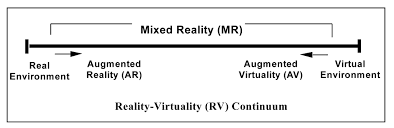
\includegraphics[width=\linewidth]{mixedrealitycontinuum}
	\caption{Mixed Reality Continuum (Source: \cite{milgram1995augmented})}
	\label{fig:mixedrealitycontinuum}
\end{figure}

Augmented reality has been defined by \textcite{azuma1997survey} as having the following three characteristics: 

\begin{enumerate}
	\item Combines real and virtual 
	\item Is interactive in real time
	\item Is registered in three dimensions
\end{enumerate} 

Virtual reality has been gaining popularity in the consumer market in recent years. It is a specific type of mixed reality featuring entirely digital visuals and virtual environments. One particular construct, augmented reality, has been gaining popularity over the years. Augmented reality refers to systems that feature predominantly real environments whose perception maybe augmented with information not readily available to the user (figure \ref{fig:augreal} for example, shows a map overlay on top of the camera view of a street). Further, some factors have been identified that help distinguish between different mixed reality systems: extent of world knowledge (whether the augmentation takes place in a modeled world or not), reproduction fidelity (quality of display of the real/virtual objects) and extent of presence metaphor (extent to which user feels they are present in the displayed scene themselves). A detailed description of mixed reality displays and differences in their characteristics can be found in \cite{milgram1995augmented}. 

\begin{figure}
	\centering
	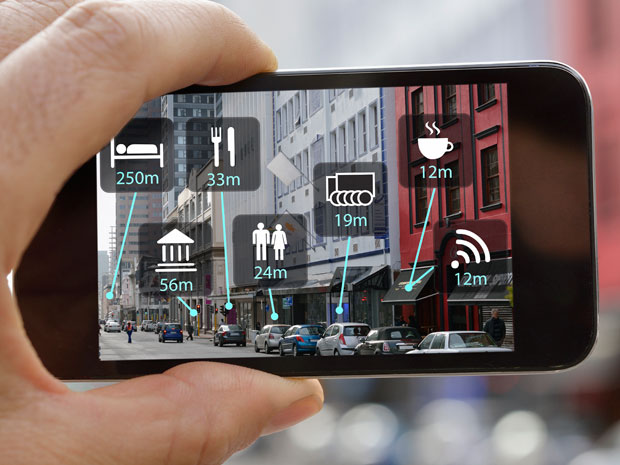
\includegraphics[width=\linewidth]{augreal}
	\caption{View of a street 'augmented' with information on places of interest}
	\label{fig:augreal}
\end{figure}

In general terms mixed reality is an emerging technology which can be used to display virtual objects merged with real world views. It has been found to be useful in job scenarios that require execution of complex tasks. A use case that has been explored in the real-world is the assembly and maintenance of equipment. Overlaying 3-D virtual guides on see-through images of actual equipment obviates the need to look away in order to refer to a manual. In the maritime sector, a study on the application of augmented reality found that 3-D virtual guides help users perform ship building and maintenance tasks in almost half the usual time \parencite{henderson2011exploring}.